\begin{flushleft}
	\section{Vista de procesos}

		La \textbf{vista de procesos} en el modelo de arquitectura \textbf{4+1} describe los \textbf{aspectos dinámicos del sistema en tiempo de ejecución}. Se enfoca en cómo se organizan y coordinan los procesos e hilos, la comunicación entre ellos y el manejo de la concurrencia, sincronización, rendimiento y escalabilidad, con el fin de satisfacer los requerimientos no funcionales del sistema.
		
		Describe cómo se organizan los procesos, cómo se comunican entre sí y cómo se comporta el sistema bajo condiciones como concurrencia, distribución, rendimiento o escalabilidad. Es especialmente útil para analizar requisitos no funcionales relacionados con el comportamiento durante la ejecución del sistema y suele representarse con diagramas UML como diagramas de actividad o de secuencia.
		
		\subsection{Diagrama de Secuencia}
		
		Basado en los \textbf{Requerimientos Funcionales} (Capítulo 3, pág. 39) y en el flujo de trabajo descrito en el \textbf{Marco Teórico} (Figura 2.2, pág. 15), la Figura \ref{fig:vista-procesos} presenta el \textbf{diagrama de secuencia} que representa el escenario principal: \textit{``El estudiante consulta su horario y navega hacia su salón usando Realidad Aumentada''}.  
		
		Este diagrama detalla la interacción entre el usuario, la interfaz de la aplicación, el motor de realidad aumentada y el backend de datos.
		
		\begin{figure}[H]
			\centering
			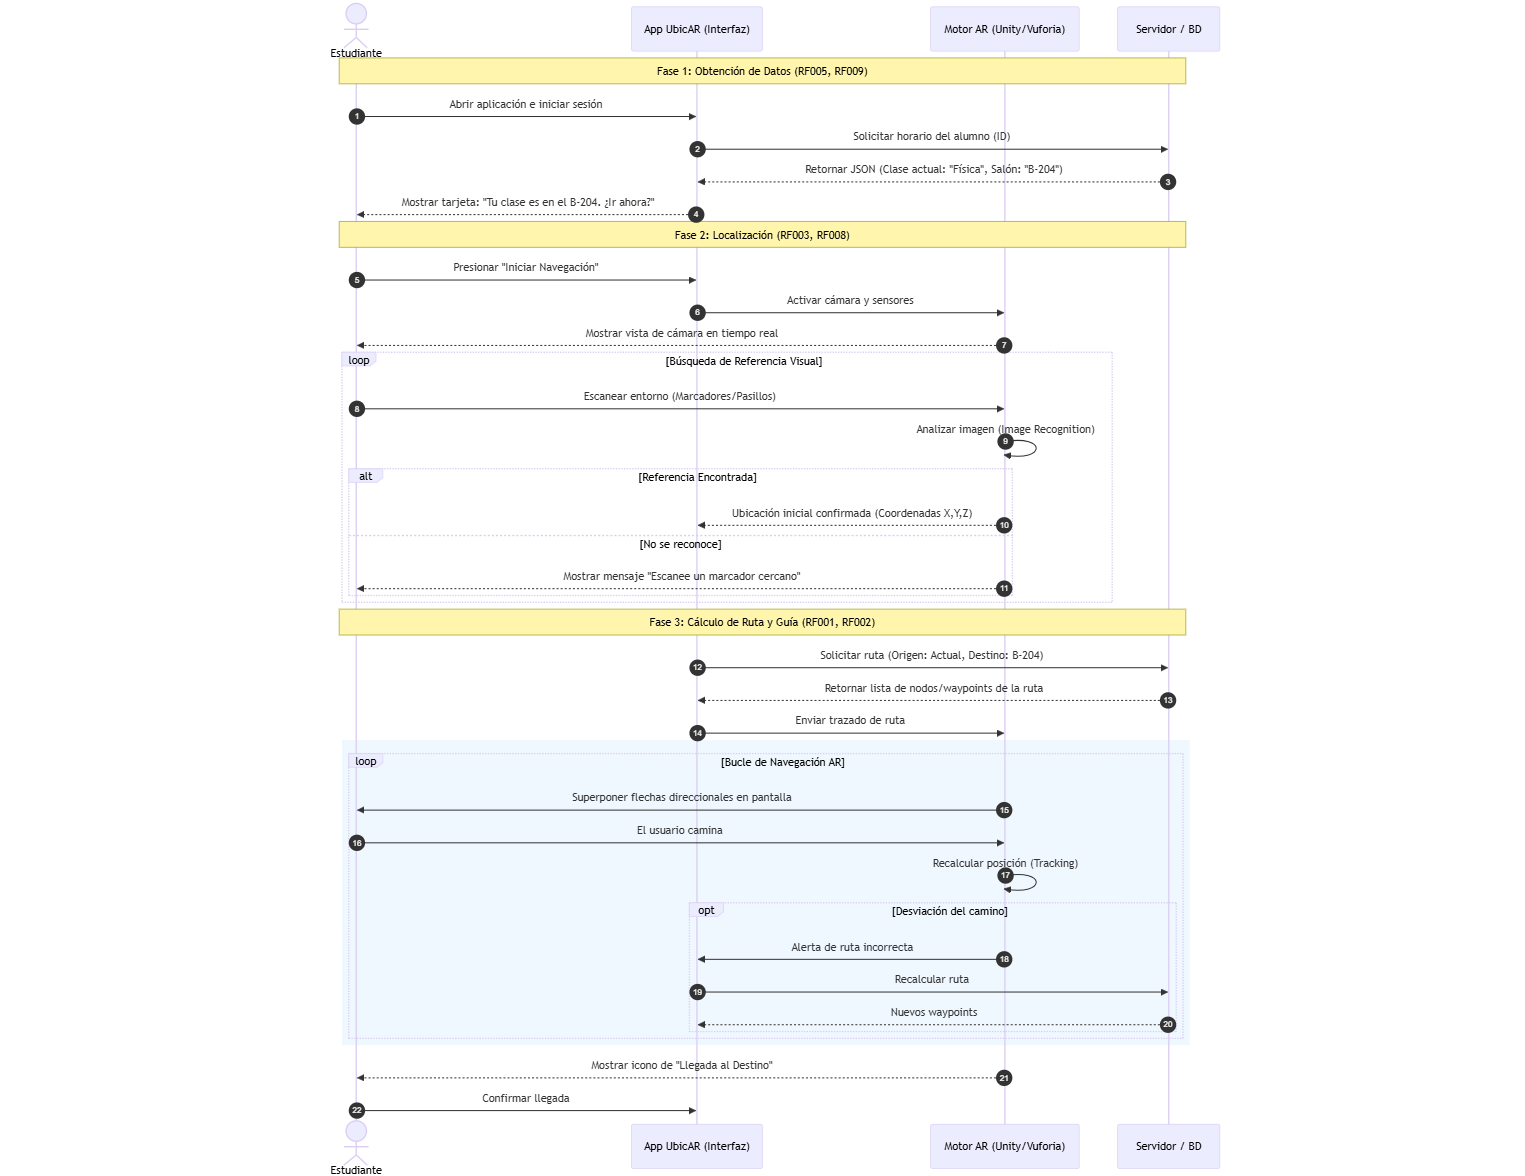
\includegraphics[width=0.95\textwidth]{imagenes/vista-procesos.png}
			\caption{Diagrama de secuencia del escenario principal de navegación con Realidad Aumentada}
			\label{fig:vista-procesos}
		\end{figure}
		
		\subsection*{Participantes}
		
		\begin{itemize}
			\item \textbf{Estudiante:} Usuario final que interactúa con la aplicación.
			\item \textbf{App UbicAR:} Capa de presentación y lógica de negocio ejecutada en el dispositivo móvil, desarrollada en \textit{Unity} con \textit{C\#}.
			\item \textbf{Motor AR:} Componente técnico responsable del procesamiento de visión por computadora y la detección del entorno, implementado mediante \textit{Vuforia} (según págs. 11 y 17).
			\item \textbf{Backend:} Servicio de datos o API que almacena la información de edificios, aulas y horarios.
		\end{itemize}
		
		\subsection*{Fases del Flujo}
		
		\begin{itemize}
			\item \textbf{Fase 1 – Obtención de Datos:}  
			Corresponde al requerimiento \textbf{RF005 (Sincronización de Horario)}. El sistema consulta el backend para obtener el horario del estudiante, permitiendo que la aplicación conozca el destino antes de que el usuario realice una búsqueda manual.
			
			\item \textbf{Fase 2 – Localización:}  
			Asociada a los requerimientos \textbf{RF003 (Detección de Ubicación)} y \textbf{RF008}. En esta fase se utiliza la tecnología de \textbf{Vuforia} para reconocer la posición del usuario dentro del edificio mediante marcadores visuales o características del entorno.
			
			\item \textbf{Fase 3 – Navegación:}  
			Representa el núcleo del sistema y cubre el requerimiento \textbf{RF001 (Guía Visual)}. Se muestra un bucle continuo en el que el usuario avanza físicamente mientras el sistema recalcula su posición y actualiza las flechas direccionales en tiempo real hasta alcanzar el destino.
		\end{itemize}
		
\end{flushleft}


